\section{Results}
\label{sec:results}

\subsection{Accuracy and retained state}
Retained bytes count the correction parameters, optimizer tensors, regression statistics, residual summaries, method-specific buffers, and blending state kept between forecasts. The count excludes the frozen base, common observation history, forecast and target buffers, and temporary workspace.

Table~\ref{tab:main_results} compares seven methods on the 96 fixed-base conditions. EPOC reduces mean MSE by 15.40\% and mean MAE by 9.35\% relative to Static while retaining a median of 6,352 B. Its paired MSE reductions relative to the $\delta$-Adapter, COSA, FAC, and OMPB are 9.55\%, 4.18\%, 0.92\%, and 6.06\%, respectively. EPOC has lower MSE in 84, 77, 58, and 91 of the 96 paired conditions. All 96 EPOC conditions improve both MSE and MAE over Static. Full ELF has the highest mean reduction from Static, 19.29\% in MSE and 12.74\% in MAE, with 474,048 median retained bytes. EPOC therefore retains about one seventy-fifth of ELF's median auxiliary state, alongside a 3.89-percentage-point smaller mean MSE reduction from Static.

\begin{table*}[!t]
\caption{Seven-method comparison on 96 matched conditions. The overview averages condition-wise reductions from Static; retained-byte multiples are relative to EPOC (6,352 B) and rounded to integers. The MSE and MAE panels average losses over three seeds and the legacy/refit variants within each series--backbone pair. The rightmost ratio divides EPOC's unrounded loss by the lowest unrounded loss in that row; 1 indicates the best result. Bold marks row-minimum losses and the corresponding ratio when EPOC is best. All corrections use global blending.}
\label{tab:main_results}
\centering
\begingroup\fontsize{9}{10.5}\selectfont
\setlength{\tabcolsep}{2.5pt}
\begin{tabular}{@{}lrrr@{}}
\toprule
\multicolumn{4}{@{}l}{\textit{96-condition overview}} \\
Method & MSE $\uparrow$ (\%) & MAE $\uparrow$ (\%) & Retained bytes $\downarrow$ \\
\midrule
Static & 0.00 & 0.00 & 0 ($\times0$) \\
$\delta$-Adapter & 6.70 & 5.12 & 22,552,608 ($\times3550$) \\
COSA & 11.73 & 7.56 & 111,756 ($\times18$) \\
FAC & 14.59 & 9.11 & 33,312 ($\times5$) \\
OMPB & 10.05 & 6.73 & 767,216 ($\times121$) \\
ELF & 19.29 & 12.74 & 474,048 ($\times75$) \\
EPOC & 15.40 & 9.35 & 6,352 ($\times1$) \\
\bottomrule
\end{tabular}
\par\vspace{5pt}
\begin{tabular}{@{}llrrrrrrrr@{}}
\toprule
\multicolumn{10}{@{}l}{\textit{MSE $\downarrow$}} \\
Dataset & Backbone & Static & $\delta$-Adapter & COSA & FAC & OMPB & ELF & EPOC & EPOC/best \\
\midrule
ETTh1 & DLinear & 0.3962 & 0.3939 & 0.3929 & 0.3840 & 0.3920 & 0.3673 & \textbf{0.3583} & \textbf{1.00000} \\
ETTh1 & PatchTST & 0.4378 & 0.4341 & 0.4143 & 0.3983 & 0.4018 & \textbf{0.3654} & 0.3779 & 1.03433 \\
ETTh2 & DLinear & 0.1453 & 0.1421 & 0.1397 & 0.1401 & 0.1414 & 0.1349 & \textbf{0.1341} & \textbf{1.00000} \\
ETTh2 & PatchTST & 0.1805 & 0.1752 & 0.1501 & 0.1407 & 0.1475 & \textbf{0.1382} & 0.1422 & 1.02896 \\
ETTm1 & DLinear & 0.2630 & 0.2570 & 0.2498 & \textbf{0.2366} & 0.2561 & 0.2390 & 0.2467 & 1.04298 \\
ETTm1 & PatchTST & 0.3167 & 0.3105 & 0.2653 & 0.2608 & 0.2793 & \textbf{0.2368} & 0.2718 & 1.14783 \\
ETTm2 & DLinear & 0.0998 & 0.0971 & 0.0960 & 0.0918 & 0.0965 & \textbf{0.0860} & 0.0895 & 1.04031 \\
ETTm2 & PatchTST & 0.1169 & 0.1120 & 0.0989 & 0.0943 & 0.0989 & \textbf{0.0862} & 0.0927 & 1.07540 \\
Appliances & DLinear & 0.2307 & 0.1994 & 0.2158 & 0.1858 & 0.2118 & 0.1932 & \textbf{0.1843} & \textbf{1.00000} \\
Appliances & PatchTST & 0.4393 & 0.3476 & 0.2018 & 0.1897 & 0.2059 & \textbf{0.1803} & 0.1827 & 1.01291 \\
BDG2 (Rat) & DLinear & 0.2193 & 0.2049 & 0.2011 & 0.1992 & 0.2062 & \textbf{0.1839} & 0.1929 & 1.04911 \\
BDG2 (Rat) & PatchTST & 0.2129 & 0.1941 & 0.1897 & 0.1857 & 0.1917 & \textbf{0.1737} & 0.1871 & 1.07681 \\
BDG2 (Fox) & DLinear & 0.2375 & 0.2024 & 0.1993 & 0.2065 & 0.2243 & \textbf{0.1761} & 0.2091 & 1.18712 \\
BDG2 (Fox) & PatchTST & 0.1817 & 0.1632 & 0.1623 & 0.1605 & 0.1689 & \textbf{0.1545} & 0.1714 & 1.10953 \\
BDG2 (Panther) & DLinear & 0.0779 & 0.0726 & 0.0715 & 0.0706 & 0.0757 & \textbf{0.0645} & 0.0666 & 1.03126 \\
BDG2 (Panther) & PatchTST & 0.0752 & 0.0689 & 0.0690 & 0.0670 & 0.0697 & \textbf{0.0642} & 0.0673 & 1.04854 \\
\bottomrule
\end{tabular}
\par\vspace{5pt}
\begin{tabular}{@{}llrrrrrrrr@{}}
\toprule
\multicolumn{10}{@{}l}{\textit{MAE $\downarrow$}} \\
Dataset & Backbone & Static & $\delta$-Adapter & COSA & FAC & OMPB & ELF & EPOC & EPOC/best \\
\midrule
ETTh1 & DLinear & 0.4040 & 0.4021 & 0.3989 & 0.3951 & 0.3984 & \textbf{0.3863} & 0.3863 & 1.00004 \\
ETTh1 & PatchTST & 0.4400 & 0.4364 & 0.4221 & 0.4122 & 0.4159 & \textbf{0.3922} & 0.4083 & 1.04097 \\
ETTh2 & DLinear & 0.2577 & 0.2538 & 0.2498 & 0.2513 & 0.2507 & 0.2443 & \textbf{0.2429} & \textbf{1.00000} \\
ETTh2 & PatchTST & 0.2974 & 0.2902 & 0.2633 & 0.2529 & 0.2596 & \textbf{0.2498} & 0.2555 & 1.02289 \\
ETTm1 & DLinear & 0.3389 & 0.3327 & 0.3263 & \textbf{0.3177} & 0.3313 & 0.3191 & 0.3266 & 1.02787 \\
ETTm1 & PatchTST & 0.3615 & 0.3555 & 0.3363 & 0.3339 & 0.3435 & \textbf{0.3182} & 0.3433 & 1.07887 \\
ETTm2 & DLinear & 0.2115 & 0.2072 & 0.2051 & 0.2009 & 0.2056 & \textbf{0.1915} & 0.1982 & 1.03468 \\
ETTm2 & PatchTST & 0.2329 & 0.2247 & 0.2097 & 0.2030 & 0.2088 & \textbf{0.1923} & 0.2030 & 1.05589 \\
Appliances & DLinear & 0.2870 & 0.2565 & 0.2788 & 0.2560 & 0.2752 & 0.2562 & \textbf{0.2491} & \textbf{1.00000} \\
Appliances & PatchTST & 0.3857 & 0.3346 & 0.2667 & 0.2604 & 0.2689 & \textbf{0.2493} & 0.2503 & 1.00408 \\
BDG2 (Rat) & DLinear & 0.3095 & 0.2869 & 0.2856 & 0.2854 & 0.2900 & \textbf{0.2659} & 0.2814 & 1.05813 \\
BDG2 (Rat) & PatchTST & 0.3140 & 0.2906 & 0.2850 & 0.2824 & 0.2876 & \textbf{0.2648} & 0.2860 & 1.08016 \\
BDG2 (Fox) & DLinear & 0.3171 & 0.2840 & 0.2888 & 0.2954 & 0.3042 & \textbf{0.2671} & 0.2993 & 1.12034 \\
BDG2 (Fox) & PatchTST & 0.2912 & 0.2698 & 0.2679 & 0.2679 & 0.2747 & \textbf{0.2568} & 0.2788 & 1.08569 \\
BDG2 (Panther) & DLinear & 0.1786 & 0.1704 & 0.1702 & 0.1692 & 0.1759 & \textbf{0.1598} & 0.1632 & 1.02153 \\
BDG2 (Panther) & PatchTST & 0.1770 & 0.1644 & 0.1655 & 0.1627 & 0.1661 & \textbf{0.1590} & 0.1647 & 1.03599 \\
\bottomrule
\end{tabular}
\endgroup

\end{table*}

Figure~\ref{fig:accuracy_storage} shows how the mean MSE reduction and retained bytes vary across the eight series and two backbones. Its connecting segments join the DLinear and PatchTST results for the same method within one series. EPOC occupies the lowest-storage end of the fitted online methods in each panel. The ranking by error varies by series. On Fox, COSA, FAC, and the $\delta$-Adapter each have lower MSE than EPOC with both backbones, as the corresponding rows of Table~\ref{tab:main_results} show. ELF has the lowest MSE for both Fox backbones and both Panther backbones, with substantially more retained state than EPOC.

\begin{figure*}[!t]
\def\xfigwd{\textwidth}
\centering
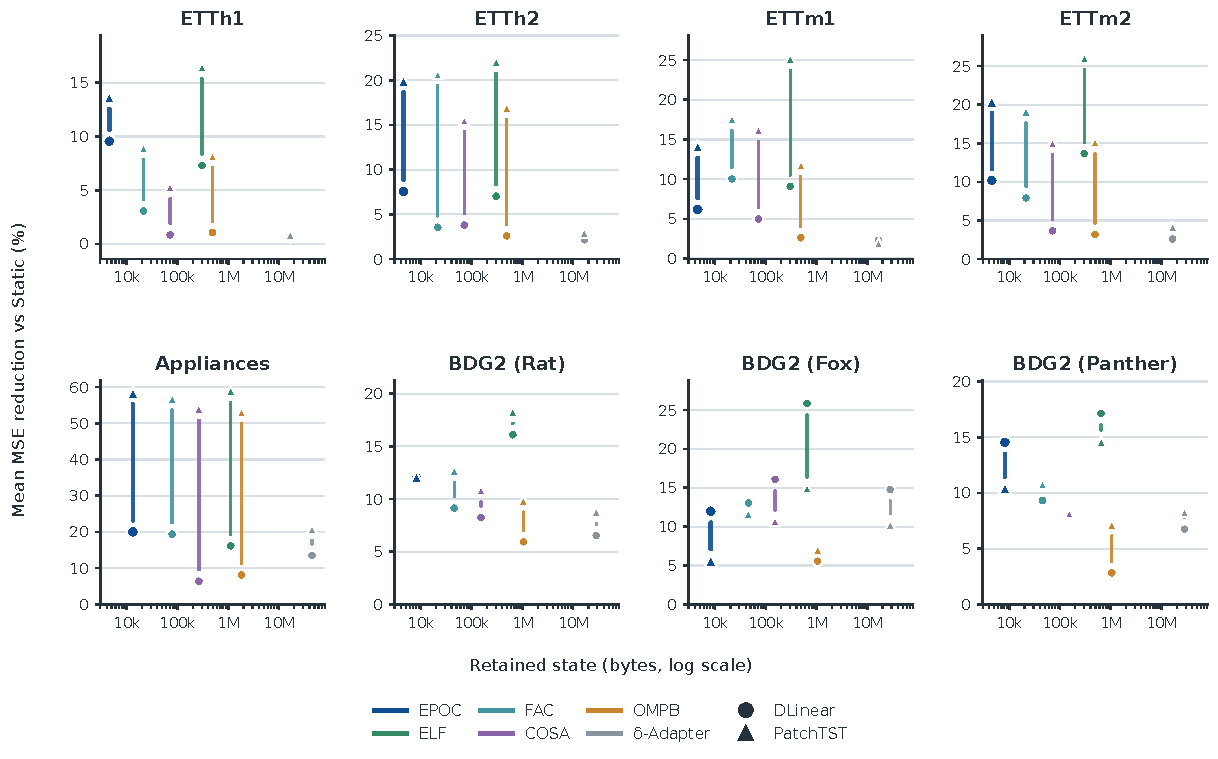
\includegraphics[width=\textwidth]{figure/fig02_accuracy_storage.pdf}
\caption{Series-level accuracy and storage for six correction methods on the 96 fixed-base conditions. Each marker averages Static-relative MSE reductions over three seeds and two training variants for one series and backbone; circles denote DLinear and triangles denote PatchTST. Lines connect the two backbones for the same method. The horizontal axis gives median retained bytes on a logarithmic scale.}
\label{fig:accuracy_storage}
\end{figure*}

Table~\ref{tab:learned_comparison} evaluates EPOC against the TEFL-style residual adapter on jointly trained bases. Across the six warmup--width settings, EPOC lowers MSE by 16.69--20.15\% and MAE by 8.82--11.29\% relative to the globally blended adapter on the \emph{same} joint base. In a separate training comparison, the raw joint adapter lowers MSE by 2.22--6.44\% relative to its paired base-only run. Thus, the direct correction comparison is made against adapters that also improve on base-only training. EPOC retains 4,528 B in each joint-base comparison. The globally blended adapters retain median sizes of 1,584 B, 1,968 B, and 13,488 B at widths 2, 4, and 64: the small adapters use less state, while the width-64 adapter uses more.

\begin{table*}[!t]
\caption{Joint-training comparison over six series, two backbones, and three seeds. The same-base columns give the paired reduction of EPOC relative to the globally blended adapter on the same jointly trained base. The separate-training columns give the reduction of the raw joint adapter relative to a separately trained base-only run. For each metric, seed losses are averaged within each of 12 series--backbone pairs before calculating reductions, which are then averaged across pairs. Retained bytes are medians for the globally blended corrections. SF denotes spectral flatness in base warmup; positive reductions favor the first-named method.}
\label{tab:learned_comparison}
\centering
\begingroup\fontsize{9}{11}\selectfont
\setlength{\tabcolsep}{4pt}
\renewcommand{\arraystretch}{1.15}
\begin{tabular}{@{}llrrrrrr@{}}
\toprule
& & \multicolumn{2}{c}{Same-base: EPOC vs. adapter} & \multicolumn{2}{c}{Separate training: adapter vs. base-only} & \multicolumn{2}{c}{Retained state (B)} \\
\cmidrule(lr){3-4}\cmidrule(lr){5-6}\cmidrule(l){7-8}
Warmup & Width & MSE (\%) & MAE (\%) & MSE (\%) & MAE (\%) & EPOC & Adapter \\
\midrule
MAE & 2 & 19.27 & 10.78 & 2.22 & 1.29 & 4,528 & 1,584 \\
& 4 & 18.98 & 10.61 & 3.13 & 1.77 & 4,528 & 1,968 \\
& 64 & 16.69 & 8.82 & 6.09 & 3.68 & 4,528 & 13,488 \\
\midrule
MAE+SF & 2 & 20.15 & 11.29 & 2.49 & 1.27 & 4,528 & 1,584 \\
& 4 & 19.54 & 10.86 & 3.68 & 1.98 & 4,528 & 1,968 \\
& 64 & 17.21 & 9.06 & 6.44 & 3.74 & 4,528 & 13,488 \\
\bottomrule
\end{tabular}
\endgroup

\end{table*}

\subsection{Endpoint selection and input construction}
Table~\ref{tab:endpoint_selection} compares equal-size residual summaries in EPOC's regression. Over the 96 fixed-base conditions, the retained endpoint lowers mean paired MSE by 2.20\%, 1.65\%, and 1.96\% relative to the first residual, middle residual, and block mean, respectively. The corresponding MAE reductions are 1.46\%, 1.11\%, and 1.39\%. The joint-base groups show the same ordering of positive endpoint gains: their MSE reductions range from 4.70\% to 6.00\% with MAE warmup and from 5.43\% to 6.94\% with MAE+SF warmup. Within each condition, the endpoint and its three controls retain the same number of bytes, so these comparisons evaluate the chosen scalar summary at fixed regression and storage size.

\begin{table*}[!t]
\centering
\caption{Endpoint gain over equal-size residual summaries. Each entry gives the mean paired reduction when the preceding block's endpoint replaces the listed first residual, middle residual, or block mean. The frozen-base row averages 96 condition-wise reductions; each joint row averages reductions across 12 series--backbone pairs after seed-mean losses are formed. All variants within a comparison use the same base, regression settings, blending rule, and retained array size.}
\label{tab:endpoint_selection}
\begingroup\fontsize{9}{11}\selectfont
\setlength{\tabcolsep}{5pt}
\renewcommand{\arraystretch}{1.18}
\begin{tabular}{@{}lrrrrrrr@{}}
\toprule
& \multicolumn{3}{c}{MSE reduction (\%)} & \multicolumn{3}{c}{MAE reduction (\%)} & \\
\cmidrule(lr){2-4}\cmidrule(lr){5-7}
Base / training & First & Middle & Mean & First & Middle & Mean & Retained (B) \\
\midrule
Frozen base (96 conditions) & 2.20 & 1.65 & 1.96 & 1.46 & 1.11 & 1.39 & 6,352 \\
Joint MAE (12 pairs) & 4.70 & 4.83 & 6.00 & 2.93 & 2.95 & 3.61 & 4,528 \\
Joint MAE+SF (12 pairs) & 5.43 & 5.49 & 6.94 & 3.38 & 3.34 & 4.14 & 4,528 \\
\bottomrule
\end{tabular}
\endgroup

\end{table*}

Figure~\ref{fig:input_ablation} tests the complete regression input on the same 96 fixed-base conditions. The complete input yields a 15.40\% mean MSE reduction from Static, compared with 13.37\% without the endpoint, 13.87\% without residual DCT coefficients, 13.02\% without current forecast coefficients, and 11.34\% with the endpoint alone. In paired losses, the complete input reduces MSE by 4.55\% relative to endpoint-only regression and wins in all 96 conditions. An endpoint projected from the retained DCT coefficients yields a 14.98\% mean MSE reduction from Static, close to the 15.40\% of the observed-endpoint variant. Supplying that projected value to all component regressions therefore recovers much of the gain obtained by explicitly sharing an endpoint input. The complete method retains 6,352 median bytes, versus 6,264 B with the projected endpoint and 2,832 B with endpoint-only regression.

\begin{figure*}[!t]
\def\xfigwd{\textwidth}
\centering
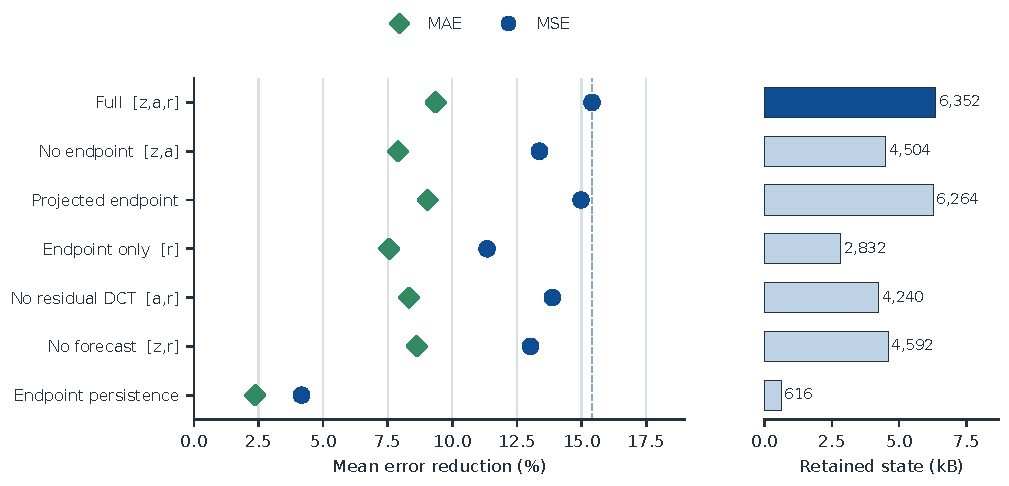
\includegraphics[width=.75\textwidth]{figure/fig05_input_ablation.pdf}
\caption{Input construction on 96 matched fixed-base conditions. Markers show mean condition-wise MSE and MAE reductions from Static; bars show median retained bytes with global blending. The projected endpoint $\tilde r$ is reconstructed from retained residual DCT coefficients and supplied to every component regression. Endpoint persistence repeats the preceding endpoint without a fitted regression.}
\label{fig:input_ablation}
\end{figure*}

\subsection{Accuracy--storage and setting sensitivity}
The upper panels of Fig.~\ref{fig:overview_sensitivity} put all six corrections from Table~\ref{tab:main_results} on common MSE, MAE, and retained-state axes. EPOC gives a 15.40\% mean MSE reduction at 6,352 median bytes; full ELF gives 19.29\% at 474,048 B. FAC is the closest of the other main comparators in mean MSE reduction, at 14.59\% and 33,312 B. These points show the accuracy and storage choices behind the paired comparisons.

The lower panels vary one EPOC setting at a time over the same 96 conditions. Increasing $K$ from 1 to 4 raises the mean MSE reduction from 11.13\% to 15.40\% and median retained bytes from 2,056 to 6,352. At $K=8$, MSE reduction reaches 16.40\% with 12,080 B. The additional 1.00 percentage point from $K=4$ to $K=8$ requires 5,728 more retained bytes. With $K=4$ fixed, changing ridge strength, forgetting half-life, or blending window produces mean MSE reductions between 14.47\% and 15.43\%. Component count is the largest accuracy--storage choice among these one-factor changes. Table~\ref{tab:s_sensitivity} gives the full 13-setting summary, with condition-level values in the accompanying CSV.

\begin{figure*}[!t]
\def\xfigwd{\textwidth}
\centering
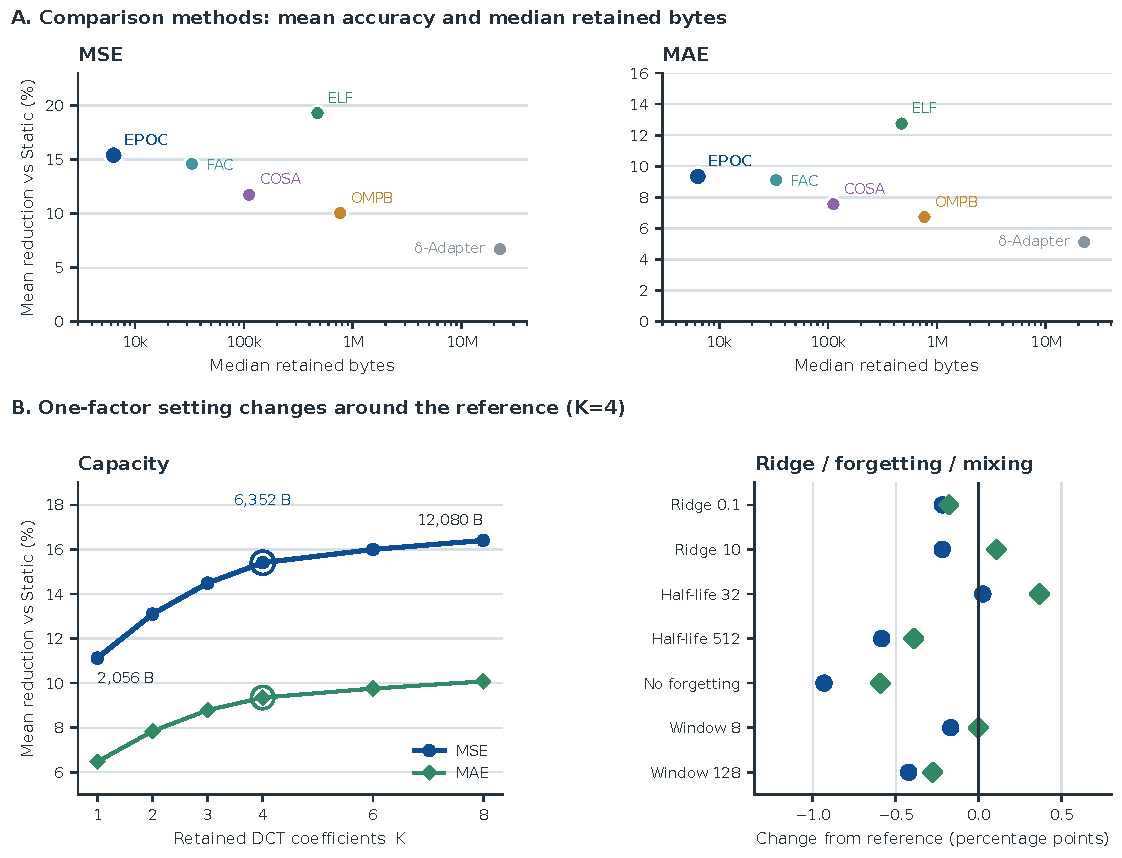
\includegraphics[width=.80\textwidth]{figure/fig06_overview_sensitivity.pdf}
\caption{Main comparison and one-factor sensitivity on 96 fixed-base conditions. Upper panels plot mean condition-wise reductions from Static against median retained bytes for the six globally blended correction methods. Lower left varies the retained DCT component count $K$; lower right changes ridge strength, forgetting half-life, or blending window relative to the $K=4$ reference. Unchanged settings follow Section~\ref{sec:method}.}
\label{fig:overview_sensitivity}
\end{figure*}
